\documentclass[11pt,lang=en]{elegantbook}

\title{Abstract Algebra Note}
% \subtitle{Classic Elegant\LaTeX{} Template}

\author{isomo}
% \institute{Elegant\LaTeX{} Program}
\date{\today}
% \version{4.5}
% \bioinfo{Bio}{Information}

% \extrainfo{\textcolor{red}{\bfseries Caution: This template will no longer be maintained since January 1st, 2023.}}

% \logo{logo-blue.png}
\cover{cover.jpg}

% modify the color in the middle of titlepage
\definecolor{customcolor}{RGB}{32,178,170}
\colorlet{coverlinecolor}{customcolor}
\usepackage{cprotect}

% \addbibresource[location=local]{reference.bib} % bib

\begin{document}

\maketitle

\frontmatter
\tableofcontents

\mainmatter



\chapter{ElegantBook Writing Sample}

\begin{introduction}
\item Theorem Class Envrionments
\item Cross Reference
\item Math Environments
\item List Environments
\item Logo and Base 
\item $a^2+b^2=c^2$
\end{introduction}


\lipsum[1]
% source: https://www.maths.tcd.ie/~dwilkins/LaTeXPrimer/Theorems.html

\section{Writing Sample}

We will define the integral of a measurable function in three steps. First, we define the integral of a nonnegative simple function. Let $E$ be the measurable set in $\mathcal{R}^N$.

\begin{definition}[Left Coset]
Let $H$ be a subgroup of a group~$G$.  A \emph{left coset} of $H$ in $G$ is a subset of $G$ that is of the form $xH$, where $x \in G$ and $xH = \{ xh : h \in H \}$. Similarly a \emph{right coset} of $H$ in $G$ is a subset of $G$ that is of the form $Hx$, where $Hx = \{ hx : h \in H \} \hbar$ 
\end{definition}

\begin{note}
Note that a subgroup~$H$ of a group $G$ is itself a left coset of $H$ in $G$.
\end{note}

\lipsum[2]

\begin{theorem}[Lagrange's Theorem] \label{thm:lg}
Let $G$ be a finite group, and let $H$ be a subgroup of $G$. Then the order of $H$ divides the order of $G$.
\end{theorem}

As theorem \ref{thm:lg} refered.

\lipsum[3]


\begin{theorem}{theorem name}{label text}
  The content of theorem.
\end{theorem}

we can refer this theorem as \ref{thm:label text}.


\begin{proposition}[Size of Left Coset]
Let $H$ be a finite subgroup of a group $G$.  Then each left coset of $H$ in $G$ has the same number of elements as $H$.
\end{proposition}

\begin{proof}
  Let $z$ be some element of $xH \cap yH$. Then $z = xa$ for some $a \in H$, and $z = yb$ for some $b \in H$. If $h$ is any element of $H$ then $ah \in H$ and $a^{-1}h \in H$, since $H$ is a subgroup of $G$. But $zh = x(ah)$ and $xh = z(a^{-1}h)$ for all $h \in H$. Therefore $zH \subset xH$ and $xH \subset zH$, and thus $xH = zH$.  Similarly $yH = zH$, and thus $xH = yH$, as required. 
\end{proof}

\begin{figure}[htbp]
  \centering
  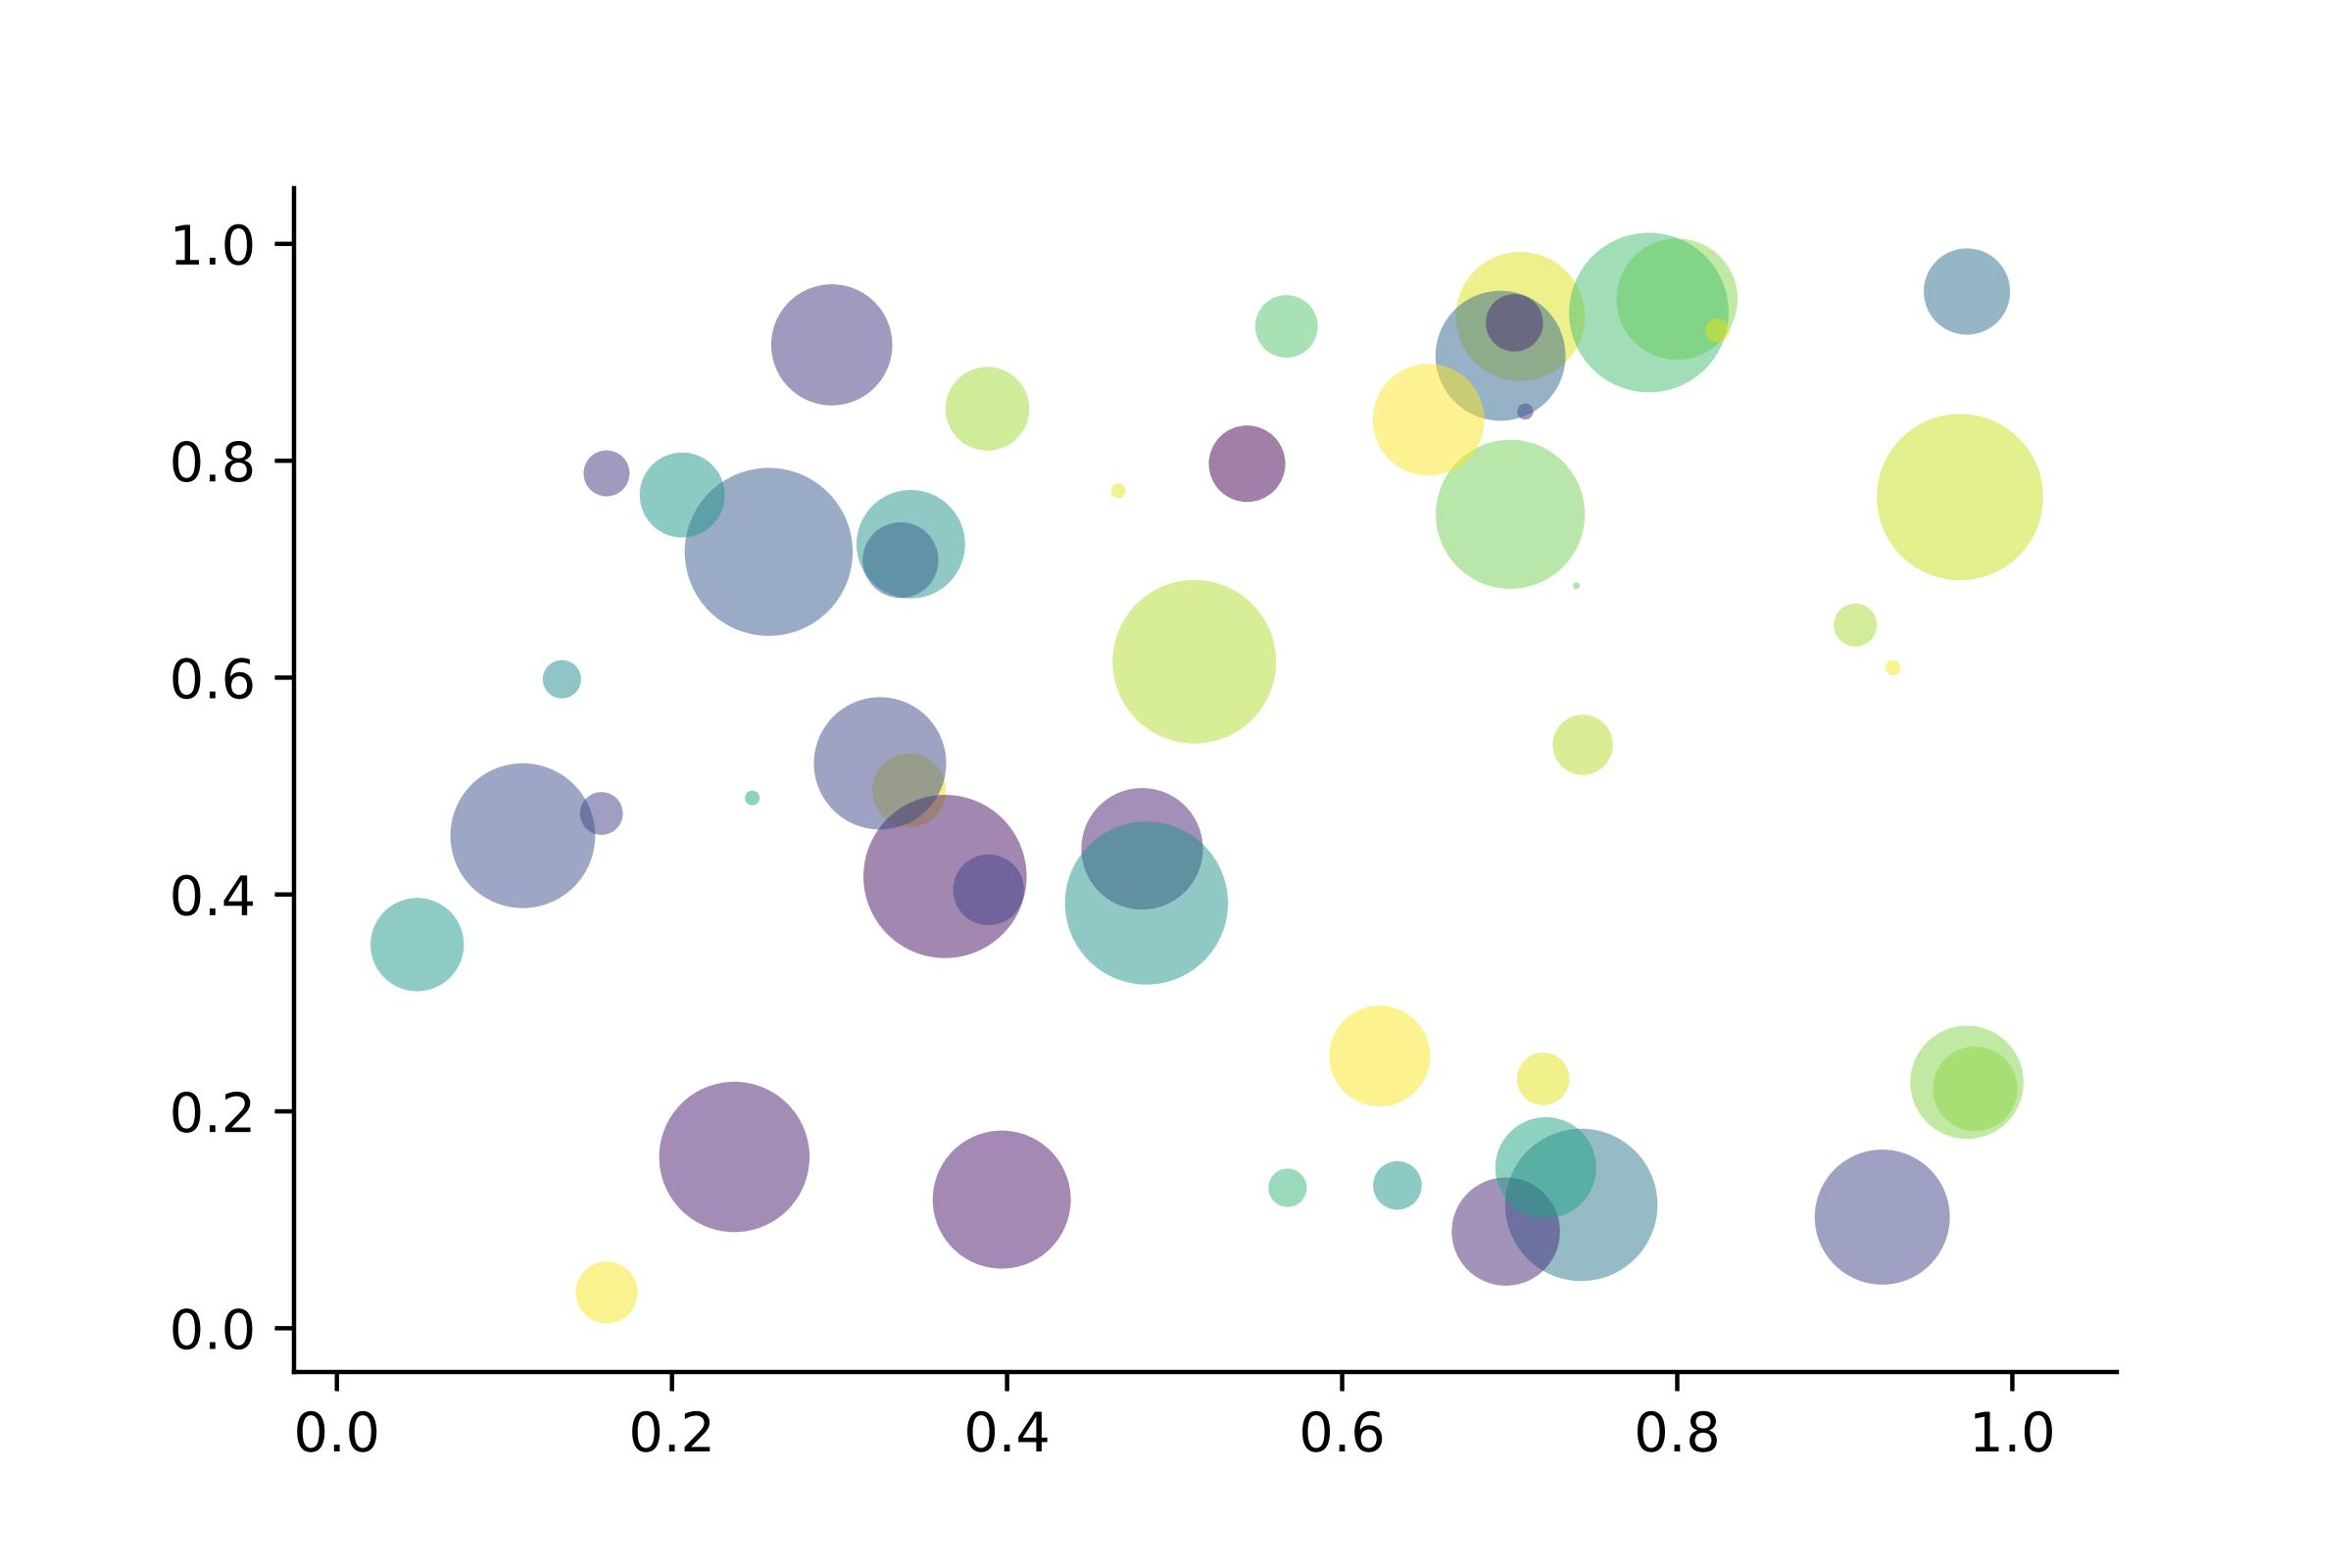
\includegraphics[width=0.6\textwidth]{scatter.jpg}
  \caption{Matplotlib: Scatter Plot Example\label{fig:scatter}}
\end{figure}

Regression analysis is a powerful statistical method that allows you to examine the relationship between two or more variables of interest. While there are many types of regression analysis, at their core they all examine the influence of one or more independent variables on a dependent variable. The process of performing a regression allows you to confidently determine which factors matter most, which factors can be ignored, and how these factors influence each other.

Let's continue using our application training example. In this case, we'd want to measure the historical levels of satisfaction with the events from the past three years or so, as well as any information possible in regards to the independent variables. 

\section{Second section}
This second section\index{S!section} may include some special word, 
and expand the ones already used\index{keywords!used}.


\begin{table}[htbp]
  \small
  \centering
  \caption{Auto MPG and Price \label{tab:reg}}
    \begin{tabular}{lcc}
    \toprule
                    &       (1)         &        (2)      \\
    \midrule
    mpg             &    -238.90***     &      -49.51     \\
                    &     (53.08)       &      (86.16)    \\
    weight          &                   &      1.75***    \\
                    &                   &      (0.641)    \\
    constant        &     11,253***     &       1,946     \\
                    &     (1,171)       &      (3,597)   \\
    obs             &        74         &         74     \\
    $R^2$           &      0.220        &       0.293    \\
    \bottomrule
    \multicolumn{3}{l}{\scriptsize Standard errors in parentheses} \\
    \multicolumn{3}{l}{\scriptsize *** $p < 0.01$, ** $p<0.05$, * $p<0.1$} \\
    \end{tabular}%
\end{table}%

\lipsum[1-2]

\begin{itemize}
  \item Routing and resource discovery;
       \begin{itemize} 
             \item Language Models
            \item Vector Space Models
         \end{itemize}
  \item Resilient and scalable computer networks;
  \item Distributed storage and search.
\end{itemize}

%\problemset



\chapter{FAQ}
We list some FAQs for users to refer to:
\begin{enumerate}
  \item \question{Why option numbers for natbib fail to take effect in v3.07?}
  In v3.07, when \lstinline{gbt7714} is introduced, option \lstinline{authoryear} is incompatible with \lstinline{natbib}. In v3.08 and 3.09, \lstinline{numbers}, \lstinline{numbers}, \lstinline{super} and \lstinline{authoryear} are introduced.
  \item \question{I want to customize font and background color.}
  Please use \lstinline{pagecolor} to change background color, refer to \href{https://tex.stackexchange.com/questions/278544/xcolor-what-is-the-equivalent-of-default-text-color}{this} to customize font.
  \item \question{Which version should I choose?}
  Please use \href{https://github.com/ElegantLaTeX/ElegantBook/releases}{Latest Release} via GitHub or \TeX{} Live 2022.
  \item \question{Which editor should I choose?}
  You can use \TeX{} Live 2022 built-in \TeX works or \TeX Studio. You may refer to \href{https://github.com/EthanDeng/texworks-autocomplete}{\TeX{}works autocomplete}. \TeX{} Live 2022 + \TeX{}studio is strongly recommended. Related configurations can be found at \href{https://github.com/EthanDeng/vscode-latex}{vscode-latex} and \href{https://github.com/EthanDeng/sublime-text-latex}{sublime-text-latex}.
  \item \question{Hello, we want to use ElegantBook to write a book about machine learning and would like your authorization.}
  Feel free to use our templates by pointing out our copyright. For other issues, please refer to LPPL-1.3c. If you want to show us your work, you can share the URL with us afterwards.
  \item \question{What is cross reference?}
  This template is aimed at who are not a complete beginner for \LaTeX{}. Please learn more about \LaTeX{} before using this template.
  \item \question{Is the language for code highlighting optional?}
  Yes, \lstinline{listings} package is used in ElegantBook, hence language is optional(e.g. \lstinline{language=Python}). For global setting, use \lstinline{lstset}. For more information, please refer to package documentations.
  \item \question{When will Beamer template (ElegantSlide or ElegantBeamer) forthcoming?}
  Since there is an excellent theme \href{https://github.com/matze/mtheme}{Metropolis}, no plan for Beamer theme.
\end{enumerate}




% \printbibliography[heading=bibintoc, title=\ebibname]
% \appendix


% \chapter{Mathematical Tools}

% This appendix covers some of the basic mathematics used in econometrics. We briefly discuss the properties of summation operators, study the properties of linear and some nonlinear equations, and review the ratios and percentages. We also introduce some special functions that are common in econometrics applications, including quadratic functions and natural logarithms. The first four sections require only basic algebraic techniques. The fifth section briefly reviews differential Calculus Although Calculus is not necessary to understand much of this book, it is used in some of the end-of-chapter appendices and in some of the more advanced topics in part 3.

% \section{Summation Operator and Description Statistics}

% \textbf{Summation Operator} is an abbreviation used to express the summation of numbers, it plays an important role in statistics and econometrics analysis. If $\{x_i: i=1, 2, \ldots, n\}$ is a sequence of $n$ numbers, the summation of the $n$ numbers is:




\end{document}